\documentclass[sigconf,article]{acmart}
\settopmatter{printacmref=false}
\renewcommand\footnotetextcopyrightpermission[1]{}
\pagenumbering{gobble}

\usepackage{booktabs}
\usepackage{amsmath}
\usepackage{graphicx}
\usepackage{microtype}
\newfontfamily\cjkfont[Path=fonts/]{DroidSansFallback-ai-cup-subset.ttf}

\begin{document}

\title[Field-Wise Metrics and Hierarchical Consistency]{When Field-Wise Metrics Miss\\
  Hierarchical Consistency: A Controlled\\
  Study on the AI CUP ESG Promise\\
  Verification Dataset}

% Author, affiliation, and email metadata are intentionally deferred until
% supplied by the submitting authors. Do not add fictional submission details.


\begin{abstract}
ESG promise verification requires jointly predicting whether text contains a
promise, its verification timeline, whether it supplies evidence,
and the quality of that evidence. These outputs obey hard dependencies, yet
the task metric scores them field by field. We conduct a controlled study of
seven decision rules using identical cross-fitted probabilities. Independent
argmax produces invalid tuples on 12.6\% of document-disjoint predictions;
deterministic projection removes them. The official weighted macro-F1 shows no
detectable projection effect ($p_{\mathrm{Holm}}=1.000$), whereas a post-hoc
path-constrained variant that changes only the treatment of
ancestor-unsupported predictions yields a positive contrast
($p_{\mathrm{Holm}}=.025$). Pre-specified tuple accuracy corroborates this
result ($p_{\mathrm{Holm}}=.001$), while uncalibrated 17-state decoding (M4)
is worse than uncalibrated projection (M1) on tuple accuracy
($p_{\mathrm{Holm}}=.028$). These
findings show that, for this dataset and backbone, field-wise scoring can
understate the utility of validity-preserving decisions.
\end{abstract}

\keywords{ESG, promise verification, hierarchical classification,
  constrained decoding, evaluation metrics}

\maketitle
\pagestyle{plain}

\section{Introduction}

ESG promise verification is not four unrelated classification problems. The
predicted promise status, verification timeline, evidence status, and evidence
quality describe one claim, and their parent--child implications determine
whether the combined output is internally usable. For example, a paragraph
predicted to contain no promise cannot coherently receive a substantive
timeline, and a prediction of no evidence cannot coherently receive an evidence
quality. Individually plausible field labels can therefore form an illegal
tuple.

The official weighted macro-F1 nevertheless scores each field separately. It
can award credit to a substantive child whose predicted ancestors do not
support that child, while a rule that preserves validity must repair or replace
it. This creates a gap between what the task structure requires and what the
ranking metric rewards. We ask whether the official field-wise score reflects
the value of enforcing the supplied hierarchy.

We study that question as a controlled decision comparison, not as a model or
competition-performance claim. Seven rules consume identical cross-fitted base
probabilities and test rows. In Chinese, the confirmatory official-score family
is null, yet pre-specified exact whole-tuple accuracy improves under projection.
We then repeat the same within-arm M1--M0 contrast across four ML-Promise
languages, four backbones per language, and two fixed training objectives.
Tuple accuracy improves in all 32 external arms, while weighted macro-F1 has a
mixed sign. This repeated pattern concerns decision contrasts within each
corpus; raw scores do not isolate language effects.

Our contributions are:
\begin{enumerate}
  \item We formalize the supplied hierarchy as 17 legal tuples out of 120 and
  audit 2,000 Chinese paragraphs from 49 companies.
  \item We compare seven decision rules on shared predictions and report the
  complete confirmatory official-score family, the pre-specified secondary
  tuple family, and adverse as well as favorable results.
  \item We externally replicate the within-arm projection contrast across four
  languages and 32 backbone-by-loss arms, while keeping post-hoc metrics and
  structural/backbone screens explicitly exploratory.
\end{enumerate}

\section{Related Work}

The AI CUP task uses the four-part formulation described in the PromiseEval
shared-task overview: identify an ESG promise, determine whether it has
actionable evidence, assess the clarity of the promise--evidence pair, and
assign a verification horizon
\cite{chen2025promiseeval}. ML-Promise is the associated
multilingual corpus resource; we use its English, French, Japanese, and Korean
releases for external replication \cite{seki2025mlpromise}. This joint
verification problem differs from
ClimateBERT-NetZero, which detects corporate and national net-zero or reduction
targets and supports analysis of their ambition, rather than jointly assessing
promise status, evidence, evidence quality, and timing
\cite{schimanski2023climatebert}.

\begingroup\emergencystretch=1em
These dependent outputs form a compact instance of hierarchical text
classification, in which labels occupy a supplied structure and coherent
predictions respect its ancestor relations \cite{plaud2024revisiting}. The AI
CUP hierarchy comes from the task's official field logic: we neither discover
the hierarchy nor propose a new hierarchical architecture. Instead, we compare
decision rules over the same field-wise probabilities while preserving or
ignoring that given structure.
\par\endgroup

Yu et al. introduced path-constrained MicroF1 and MacroF1, under which a
correct node receives credit only when all its ancestors are also correct
\cite{yu2022constrained}. Ji et al. later named this family \emph{C-metrics}
\cite{ji2023hierarchical}. Our path-constrained weighted macro-F1 (C-wF1)
adapts Yu et al.'s principle to this task's fields and its official
weighted macro-F1; it is therefore not the original C-MacroF1.
Section~\ref{sec:metrics} defines both it and the set-overlap hierarchical
F1 (hF). Both were adopted post hoc and are reported as exploratory.

Plaud et al. observed from point estimates that constrained F1 variants did not
globally change method rankings in their experiments
\cite{plaud2024revisiting}. That observation and our post-hoc paired contrast
inference answer different questions: ranking a collection of models is not the
same estimand as a paired difference between decision rules on shared rows and
probabilities. Moreover, our hF changes both consistency treatment and
macro-versus-micro aggregation. Of the two post-hoc metrics, only C-wF1
isolates the treatment of children whose predicted ancestors do not
support them, while retaining
the official field aggregation.

\section{Task and Data}

\paragraph{Outputs and legal states.}
The task predicts four fields for each paragraph. We study the AI CUP
VeriPromise\hspace{0pt}ESG development release.
Promise status (PS) is \emph{Yes} or \emph{No}. Verification timeline (VT) is
\emph{already}, \emph{within two years}, \emph{between two and five years},
\emph{more than five years}, or \emph{N/A}. Evidence status (ES) is
\emph{Yes}, \emph{No}, or \emph{N/A}; evidence quality (EQ) is \emph{Clear},
\emph{Not Clear}, \emph{Misleading}, or \emph{N/A}. These fields obey hard
implications: PS=No requires VT=ES=EQ=N/A, whereas PS=Yes requires one of the
four substantive timelines and ES in \{Yes, No\}. In turn, ES=No requires
EQ=N/A, whereas ES=Yes requires one of the three substantive quality labels.
Thus the Cartesian label space has $2\times5\times3\times4=120$
combinations, but only
\begin{equation}
  1+4(1+3)=17
  \label{eq:legal-states}
\end{equation}
legal tuples: one for PS=No, and for each of four timelines either one ES=No
state or three ES=Yes quality states.

\begin{figure*}[t]
  \centering
  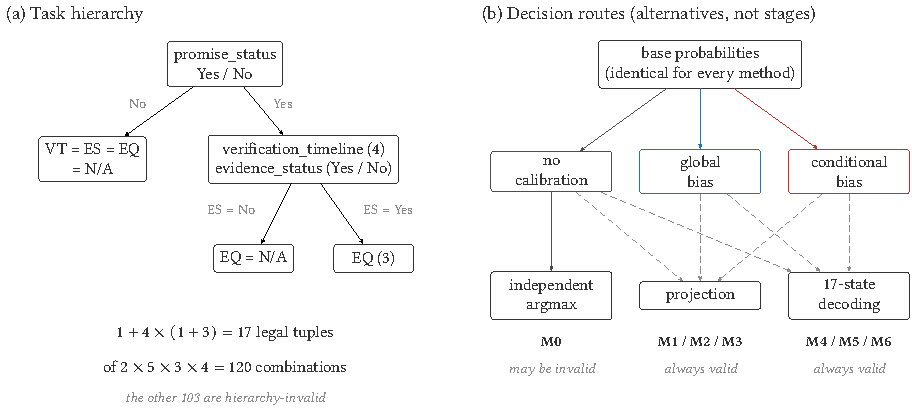
\includegraphics{../figures/figure1_hierarchy.pdf}
  \caption{The task hierarchy and the alternative decision routes. All routes
  consume identical base probabilities; projection and 17-state decoding
  guarantee a legal tuple, whereas independent argmax does not.}
  \label{fig:hierarchy}
\end{figure*}

\paragraph{Development-set audit.}
The release contains 2,000 labeled development paragraphs from 49 source
reports covering 50 companies, and it realizes 15 of the 17 legal states
(Table~\ref{tab:dataset}). The rarest EQ label,
\emph{Misleading}, has only two instances; we therefore make no improvement
or significance claim for that class.

\begin{table}[t]
  \centering
  \caption{Dataset summary from the frozen study artifact.}
  \label{tab:dataset}
  \begin{tabular}{lrr}
\toprule
Statistic & Development & Competition test \\
\midrule
Paragraphs & 2000 & 2000 \\
Source reports (PDFs) & 49 & 49 \\
\quad shared with other split & 49 & 49 \\
Companies & 49 & 49 \\
Gold labels available & Yes & No \\
Gold hierarchy-valid tuples & 2000 / 2000 & n/a \\
Legal states observed & 15 / 17 & n/a \\
\midrule
\multicolumn{3}{l}{\emph{Rarest classes}} \\
\quad within\_2\_years & 34 & n/a \\
\quad Misleading & 2 & n/a \\
\bottomrule
\end{tabular}

\end{table}

All 49 development reports also occur in the unlabeled competition test data,
and one paragraph text occurs in both splits. This overlap describes sources
and text only: because competition test labels are unavailable, we infer no
label-derived test statistic. No company contributes more than one report;
one report covers two companies. Consequently, in this corpus a
document-disjoint split is necessarily company-disjoint, rather than a
separate company-level experiment.

\section{Methods}

The controlled comparison applies seven decision rules to the same
cross-fitted base probabilities, separating decision-time constraints from
model probabilities.

\begin{figure*}[t]
  \centering
  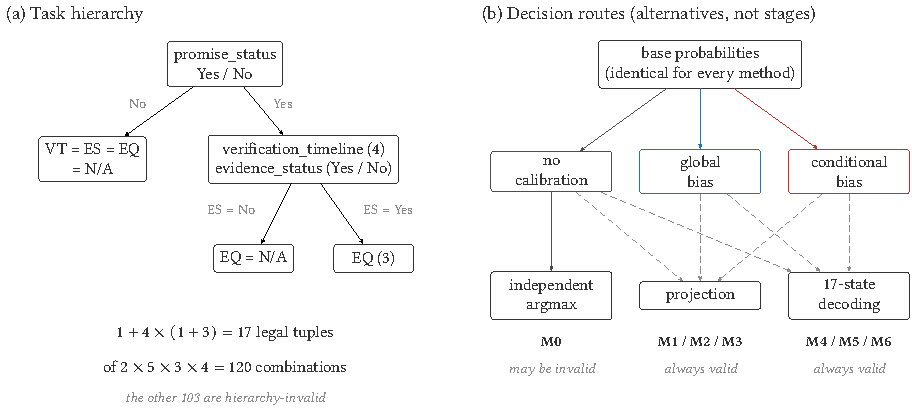
\includegraphics[width=0.9\textwidth]{../figures/figure1_hierarchy.pdf}
  \caption{Hierarchy of the four task outputs.}
  \label{fig:hierarchy}
\end{figure*}

\section{Experiments}

The primary estimand uses document-disjoint evaluation and reports all tested
decision rules from the frozen controlled study.

\begin{table*}[t]
  \centering
  \small
  \caption{Main document-disjoint results from the frozen study artifact.}
  \label{tab:main-results}
  \begin{tabular}{llrrrrrrrr}
\toprule
ID & Calibration & Decoding & wF1 (official) & PS & VT & ES & EQ & Tuple acc. & Invalid \% \\
\midrule
M0 & None & Independent & 0.572$\pm$0.003 & 0.796 & 0.464 & 0.650 & 0.424 & 0.359$\pm$0.007 & 12.55 \\
M1 & None & Projection & 0.571$\pm$0.003 & 0.796 & 0.467 & 0.651 & 0.418 & 0.394$\pm$0.004 & 0.00 \\
M2 & Global & Projection & 0.574$\pm$0.004 & 0.796 & 0.493 & 0.650 & 0.418 & 0.428$\pm$0.004 & 0.00 \\
M3 & Conditional & Projection & 0.575$\pm$0.003 & 0.796 & 0.501 & 0.651 & 0.416 & 0.432$\pm$0.004 & 0.00 \\
M4 & None & 17-state & 0.571$\pm$0.005 & 0.799 & 0.468 & 0.648 & 0.420 & 0.388$\pm$0.003 & 0.00 \\
M5 & Global & 17-state & 0.576$\pm$0.001 & 0.796 & 0.493 & 0.649 & 0.423 & 0.430$\pm$0.001 & 0.00 \\
M6 & Conditional & 17-state & 0.567$\pm$0.008 & 0.784 & 0.494 & 0.634 & 0.418 & 0.427$\pm$0.005 & 0.00 \\
\bottomrule
\end{tabular}

\end{table*}

\section{Results}
\label{sec:results}

\begin{table*}[t]
  \centering
  \small
  \caption{Chinese paired contrasts on four metrics. Official wF1 and tuple
  accuracy are separate pre-specified Holm families of five. C-wF1 and hF were
  added post hoc; their displayed adjusted values are exploratory and support
  no claim. Intervals are uncorrected 95\% report-cluster bootstrap intervals.}
  \label{tab:contrasts}
  \begin{tabular}{llrrr}
\toprule
Metric & Contrast & $\Delta$ & 95\% CI & $p_{\mathrm{Holm}}$ \\
\midrule
Weighted macro-F1 (official) & M1-M0 & -0.001 & [-0.006, 0.003] & 1.000 \\
 & M3-M2 & -0.001 & [-0.006, 0.004] & 1.000 \\
 & M4-M1 & +0.000 & [-0.005, 0.005] & 1.000 \\
 & M6-M3 & -0.007 & [-0.017, 0.003] & 0.643 \\
 & M6-M5 & -0.009 & [-0.017, -0.001] & 0.135 \\
\midrule
Path-constrained wF1 & M1-M0 & +0.004 & [0.001, 0.007] & \textbf{0.025} \\
 & M3-M2 & -0.001 & [-0.006, 0.004] & 1.000 \\
 & M4-M1 & +0.000 & [-0.005, 0.005] & 1.000 \\
 & M6-M3 & -0.007 & [-0.017, 0.003] & 0.482 \\
 & M6-M5 & -0.009 & [-0.017, -0.001] & 0.108 \\
\midrule
Hierarchical F1 (hF) & M1-M0 & +0.003 & [0.001, 0.005] & \textbf{0.017} \\
 & M3-M2 & +0.002 & [-0.001, 0.005] & 0.302 \\
 & M4-M1 & +0.004 & [0.000, 0.007] & 0.135 \\
 & M6-M3 & +0.006 & [0.000, 0.012] & 0.151 \\
 & M6-M5 & +0.004 & [-0.001, 0.009] & 0.302 \\
\midrule
Tuple accuracy & M1-M0 & +0.035 & [0.028, 0.043] & \textbf{0.001} \\
 & M3-M2 & +0.002 & [-0.003, 0.007] & 0.973 \\
 & M4-M1 & -0.006 & [-0.010, -0.002] & \textbf{0.028} \\
 & M6-M3 & -0.005 & [-0.014, 0.004] & 0.973 \\
 & M6-M5 & -0.004 & [-0.012, 0.004] & 0.973 \\
\bottomrule
\end{tabular}

\end{table*}

\begin{figure*}[t]
  \centering
  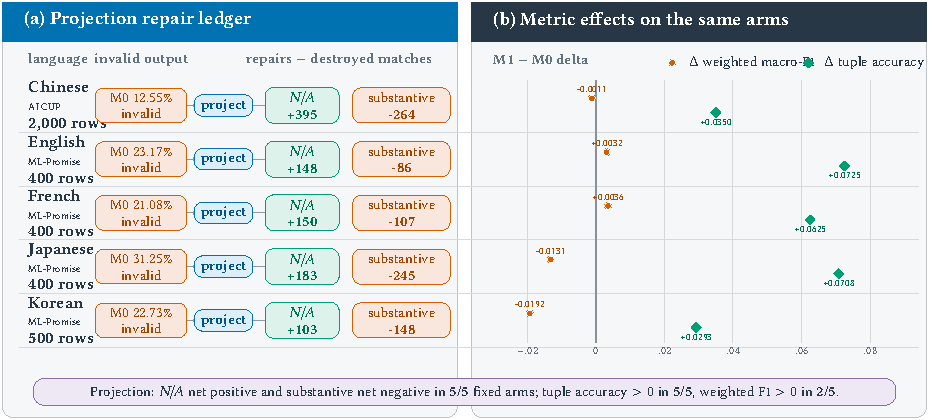
\includegraphics{../figures/figure2_multilingual.pdf}
  \caption{Multilingual projection effects in fixed document-disjoint arms.
  Each row is the preselected $\lambda=0$ M1--M0 arm. Rates and score deltas
  are means over three seeds; repair nets pool the same seeds. Equal-sized
  ledger cards encode signs and exact counts, not comparable magnitudes across
  differently sized corpora. ML-Promise wF1 applies AI CUP weights and is not
  an official ML-Promise metric.}
  \label{fig:multilingual}
\end{figure*}

\paragraph{Chinese confirmatory family.}
Table~\ref{tab:main-results} compares decision rules on identical base
probabilities and Test rows. Independent argmax (M0) produces invalid tuples
for 12.55\% of document-disjoint predictions; projection and 17-state decoding
(M1--M6) reduce this rate to zero by construction. The $\pm$ values are sample
standard deviations across the three seeds. Because each seed determines both
fold assignment and training randomness, they describe spread over the whole
split-and-training pipeline, not a confidence interval.

All five official wF1 contrasts are undetected after Holm correction. For the
central M1--M0 contrast, $\Delta=-0.001$ with 95\% interval
$[-0.006,0.003]$ and $p_{\mathrm{Holm}}=1.000$. This is absence of a detected
difference; it does not establish a zero effect.

\paragraph{Pre-specified tuple family.}
Exact whole-tuple accuracy tells a different story. M1--M0 is $+0.035$
$[0.028,0.043]$, $p_{\mathrm{Holm}}=.001$. Conversely, joint legal-state
decoding is not uniformly better: M4--M1 is $-0.006$
$[-0.010,-0.002]$, $p_{\mathrm{Holm}}=.028$. Searching every legal state can
therefore reduce whole-row correctness relative to greedy projection.

The post-hoc C-wF1 and hF M1--M0 point estimates are also positive
($+0.004$ and $+0.003$), but they do not alter the inferential hierarchy. In
the same-document sensitivity analysis, C-wF1 remains positive at $+0.002$,
while its interval $[-0.001,0.005]$ crosses zero.

\paragraph{Multilingual replication.}
Figure~\ref{fig:multilingual} fixes one arm per language before inspecting
scores. Each uses document-disjoint evaluation and $\lambda=0$.

Across all four external corpora and their four backbones at both loss
settings, M1--M0 tuple accuracy is positive in $32/32$ arms. The weighted
macro-F1 contrast is positive in only $14/32$: English $7/8$, French $5/8$,
Japanese $0/8$, and Korean $2/8$. These are within-arm directions, not a raw
score ranking across languages. For the pre-registered fixed English arm, the
one-sided report-cluster bootstrap tuple effect is $+0.0725$
$[0.0452,0.1019]$ ($p=.0002$; nine report clusters). ML-Promise weighted
scores use AI CUP weights applied to ML-Promise (not official).

\paragraph{Exploratory robustness.}
On the Chinese anchor, training-time structural loss lowers M0 invalidity from
12.55\% to 5.18\%, but its pre-registered M1 wF1 effect is only $+0.00250$
$[-0.00384,0.00860]$ ($p=.427$). Across the 16 external backbone pairs,
structural loss lowers invalidity in $16/16$, while downstream wF1 and tuple
effects are mixed. Chinese DeBERTa and ELECTRA screens likewise reduce
invalidity without a conclusive wF1 gain. Chinese RoBERTa-base emits fewer,
not more, invalid tuples than the large anchor, falsifying the simple
smaller-model mechanism. These screens are descriptive and exploratory.
\FloatBarrier

\section{Discussion}

The practical contribution of projection is its guarantee rather than a
universal field-score gain: as a retraining-free layer over compatible
field-wise probabilities, it enforces the supplied hierarchy in every arm and
improves exact whole-tuple accuracy throughout the executed external matrix,
without any claim about the underlying encoder.

\subsection{Why the two metrics disagree}
\label{sec:mechanism}
This guarantee is not cost-free in every scoring view, and
Table~\ref{tab:multilingual} makes the trade-off explicit by counting the
correct field predictions projection creates against those it destroys.
The $N\!/\!A$ net is positive and the
substantive-class net negative in all five fixed arms. If an independently
predicted parent is wrong, projection may replace a correct substantive child
with the structurally required \emph{N/A}; when the parent is correct, the same
operation can repair an unsupported child. Field-wise macro-F1 values these
changes class by class, whereas tuple accuracy credits only four-field
agreement. The field-score effect therefore varies across backbones and
corpora. Post-hoc C-wF1 and hF point in the tuple direction, but were chosen
after the primary analysis and are not needed to establish the pre-specified
secondary result.

Validity alone also does not identify the better structured rule. In Chinese,
M4 scores all 17 legal states jointly yet loses tuple accuracy to greedy M1.
Joint search can improve one field while changing another field that projection
had already made correct. This adverse result cautions against treating a
larger legal-state search as automatically superior; it does not imply that
joint decoding must fail on other models or tasks.

\subsection{Reproducibility}
\label{sec:repro}
Code, pre-registration documents, row-level predictions for all five corpora,
and the pipeline that regenerates every table here are at \url{\repourl}.

\begin{sloppypar}
\paragraph{Checkpoints.} Every backbone is a pinned Hugging Face checkpoint,
its commit revision recorded in the released configuration. Chinese:
\hfid{hfl/chinese-roberta-wwm-ext-large} (anchor),
\hfid{hfl/chinese-roberta-wwm-ext},
\hfid{IDEA-CCNL/Erlangshen-DeBERTa-v2-320M-Chinese},
\hfid{hfl/chinese-electra-180g-large-discriminator}. English:
\hfid{roberta-large}, \hfid{roberta-base},
\hfid{microsoft/deberta-v3-large},
\hfid{google/electra-large-discriminator}. French, Japanese and Korean:
\hfid{FacebookAI/xlm-roberta-large}, \hfid{FacebookAI/xlm-roberta-base},
\hfid{google/rembert}, \hfid{google-bert/bert-base-multilingual-cased}.
\end{sloppypar}

\paragraph{Procedures given only in outline above.} The document-disjoint
split sorts reports by identifier, shuffles them under the seed, re-sorts by
descending row count with a stable sort so the shuffle survives ties, then
assigns each report uniformly at random to one of the two currently lightest
folds, ties broken by fold index. Korean pages come from Poppler's \hfid{pdftotext -f P -l P -layout}, one page per labelled
(URL, page) pair, falling back to \hfid{pdftoppm -r 250} and Tesseract
(\hfid{-l kor+eng}) for image-only pages; the release already carries one
label tuple per unique (URL, page), so no further deduplication applies.
Python 3.10.20, PyTorch 2.2.2+cu121 and Transformers 4.40.2 on Linux; the 32
external arms consumed 25.4 GPU-hours in total on a single RTX 3090.

\subsection{Limitations}
The corpora differ in language, reports, annotation distributions, and primary
backbones, so the replication matrix is not a factorial estimate of a pure
language effect. English and French each have only nine report clusters, and
even Chinese inference resamples just 49. The $32/32$ and $14/32$ summaries
are therefore descriptive directions across executed arms, not a pooled
significance test. AI CUP weights applied to ML-Promise are not an official
ML-Promise metric.

Every contrast here is measured against M0, the unconstrained argmax over our
own probabilities. That is the right comparator for the question we ask, since
it holds rows and probabilities fixed, but the paper therefore reports no
comparison against a published system, an official baseline, or a leaderboard,
and nothing here is a claim about where this system ranks among participants.

Korean has a further input mismatch: its 500 examples are first-384-token PDF
pages rather than released paragraphs, and it has no gold \emph{Misleading}
example. We do not redistribute the extracted Korean text or source PDFs.
The reported Korean predictions are released and can therefore be rescored,
but retraining requires rebuilding the page inputs from their source documents
with the recipe in Section~\ref{sec:repro}.

\begin{sloppypar}
Results for structural loss and other backbones remain exploratory: they show
that reducing the invalid-tuple rate need not yield a conclusive gain on the
official score, but the fixed loss weights and limited checkpoint set cannot
characterize all training objectives or architectures. The rarest Chinese
quality label has two examples and Korean has none, so no class-level claim is
licensed for it. Finally, each seed jointly changes folds and optimization
randomness, so those two sources of variation cannot be separated.
\end{sloppypar}

\section{Conclusion}

Hierarchical projection is not a guaranteed route to higher field-wise
weighted macro-F1. It is instead a retraining-free validity layer that
eliminates invalid tuples by construction and
improves exact whole-tuple accuracy on the Chinese anchor and in all 32
evaluated external arms.
Its field-score effect varies across models and corpora, but its logical guarantee does not.
For audit-oriented tasks with dependent outputs, field-wise performance,
whole-tuple correctness, and structural validity should be reported
together.


\clearpage
\bibliographystyle{ACM-Reference-Format}
\bibliography{references}

\end{document}
